\chapter{Recommender Systems} \label{app:recommendation}
\graphicspath{{appendix/}}
Broadly speaking, the recommender systems are based on two popular strategies: the content-based filtering and the collaborative filtering. In the following, we overview the basic concepts about those techniques. 

\section{Content-based Recommendation}               \label{sec:content-recommendation}
The content-based systems exploit the attributes characterizing an item or a user. They analyze the content information collected explicitly or implicitly to construct a user or an item profile. The matching between both profiles can be quantified using a variety of similarity distances such as Cosine similarity, Pearson correlation and Latent Semantic Analysis~\cite{Deerwester:ASIS90}. This kind of matching is also applied to discover people sharing similar interests. It is closely related to detecting documents of similar content in information retrieval field. A known successful realization of content-based filtering is the Music Genome Project which is used for the Internet radio service Pandora.com. In this project, a trained music system ranks each song  based on hundreds of distinct musical characteristics. These attributes or genes capture not only a song's musical identity but also many significant qualities which are relevant to understanding listeners' musical preferences~\cite{Koren:ICS2009}. Another interesting study proposed by Chen at al.~\cite{Chen:ICHF2009} compare different recommender algorithms in the IBM's enterprise social networking service called ``Beehive''. The authors underline that the pure content matching is the most effective to recommend unknown friends and in general diverse items. However, the  content-based recommendation has the drawback to not take into account the information in preference similarity across individuals.

\section{Collaborative Filtering Recommendation}               \label{sec:collaborative-filtering}
The second strategy of recommender system is based on collaborative filtering(CF), a technique that does not need an explicit content profiling and purely rely on past user behavior~\cite{Herlocker:CSCW00}. It has been widely applied in many well-known services such as Amazon, Faceboook, LinkedIn, MySpace and Last.fm. The basis is to analyze the relationships between users and inter-dependencies among items to identify new user-item associations. In other words, the system makes automatic predictions (filtering) about the user interests based on the preferences of like-minded and similar users (collaborating). The intuition behind is that if a person A has the same preference as a person B on an item, A is more likely to have B's preference on another item, as illustrated in Figure~\ref{fig:user-cf}.

\begin{figure}[H]
  \centering
  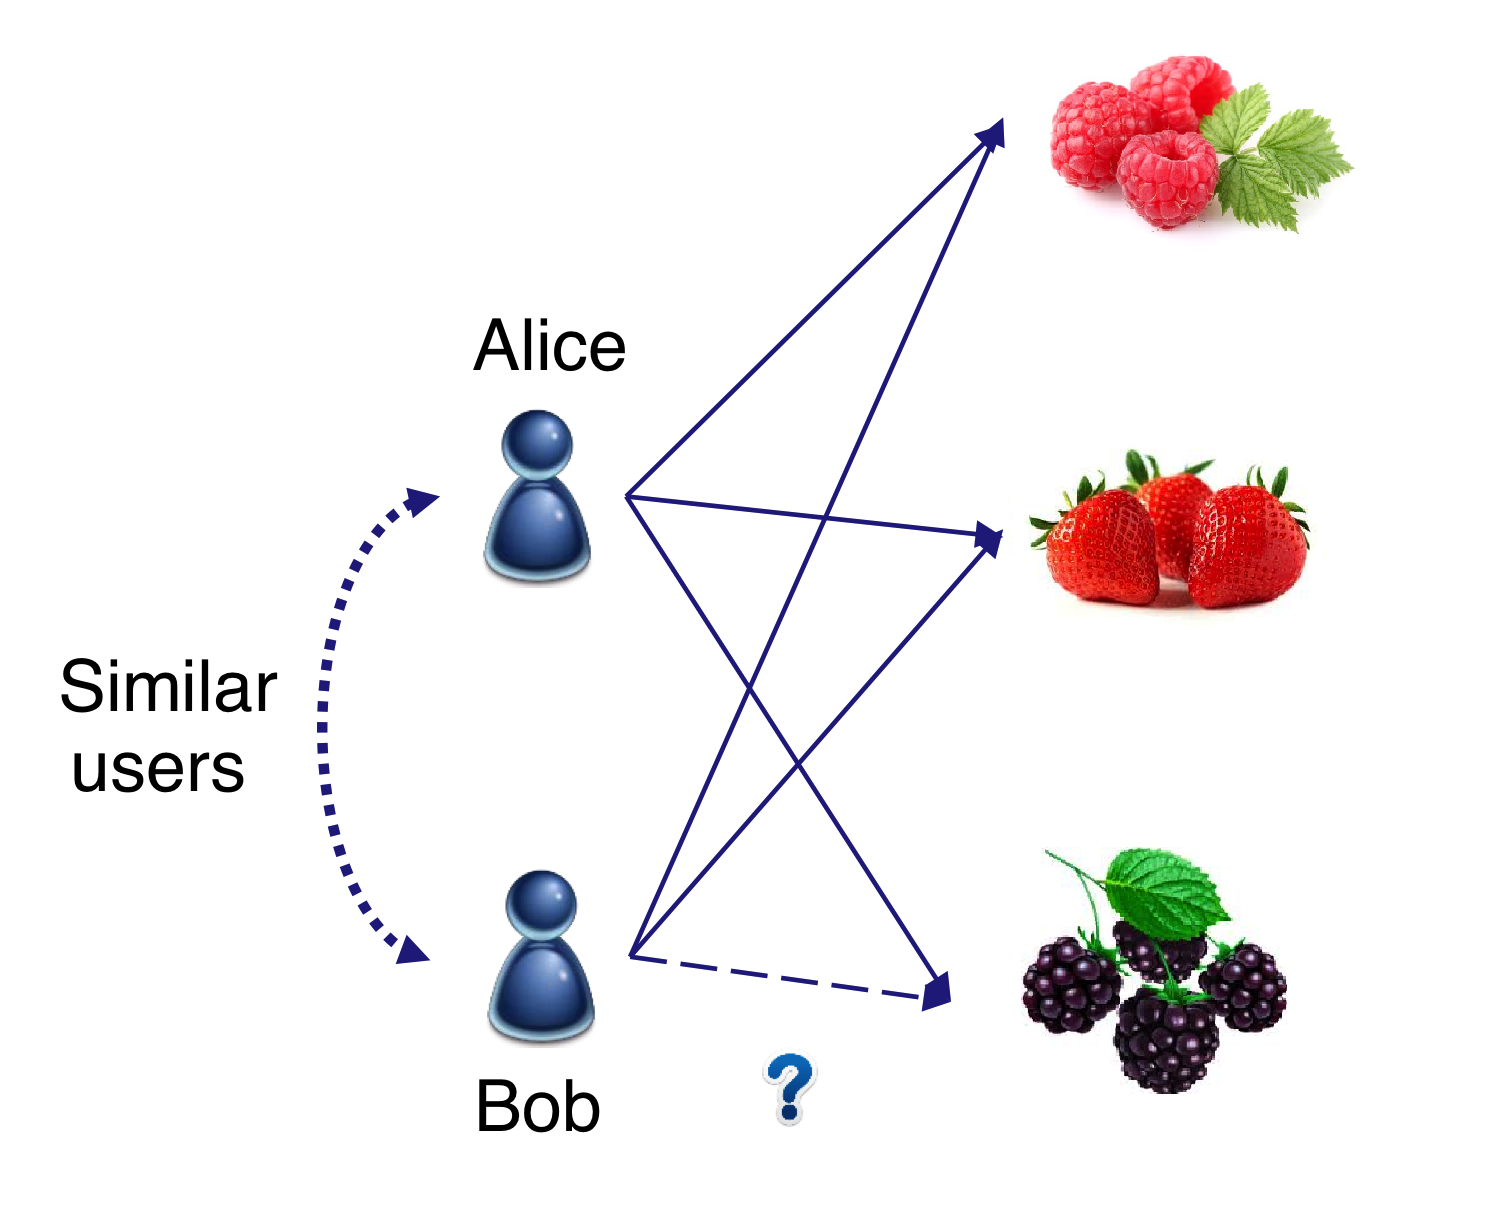
\includegraphics[scale=0.15]{user-cf.png}
  \caption{user-based collaborative filtering: Alice has a crush on berry fruits, Bob also likes two of them. The recommender system understands that Alice and Bob have similar tastes, and Bob is recommended the Blackberry}
  \label{fig:user-cf}
\end{figure}

There exists two primary categories of collaborative filtering which are memory-based and model-based approaches. The memory-based systems compute the similarity between users or, alternatively, between items based on users preferences data, thus detecting the neighbors of a given user or item. Indeed, the unknown rating value of the active user \emph{u} for an item \emph{m} is an aggregation of the ratings of users similar to \emph{u} for the same item \emph{m}, or an aggregation of the ratings of the user \emph{u} to similar items of \emph{m}. The model-based systems, on the other hand, use data mining and machine learning algorithms to estimate or learn a model from observed ratings to make predictions. A typical example is the latent factor model that discovers unobserved factors from ratings patterns. The underlying assumption is that there is a set of common hidden factors which explain a set of observations in co-occurrence data. More precisely, the similarity between users and items is simultaneously induced by some hidden lower-dimensional structure in the data. Recently, several matrix factorization methods~\cite{Koren:ICS2009} have been proposed as a successful realization of latent factor model. The users and items are simultaneously represented as unknown feature vectors within a user-item matrix. These feature vectors are learnt using low-rank approximations, so that they approximate the known preference ratings with respect to some loss measure. Despite the important success of collaborative filtering, it still suffers from three serious limitations: the sparsity problem where there are few ratings about items, the cold-start problem where items have no ratings, and the scalability where a large amount of users and items have to be analyzed.